\documentclass{article}
\usepackage[catalan]{babel}
\usepackage[latin1]{inputenc}   % Permet usar tots els accents i car�ters llatins de forma directa.
\usepackage{enumerate}
\usepackage{amsfonts, amscd, amsmath, amssymb}
\usepackage{fancyheadings}
\usepackage{graphicx}

\setlength{\textwidth}{16cm}
\setlength{\textheight}{24cm}
\setlength{\oddsidemargin}{-0.3cm}
\setlength{\evensidemargin}{0.25cm} \addtolength{\headheight}{\baselineskip}
\addtolength{\topmargin}{-3cm}

\newcommand\Z{\mathbb{Z}}
\newcommand\R{\mathbb{R}}
\newcommand\N{\mathbb{N}}
\newcommand\Q{\mathbb{Q}}
\newcommand\K{\Bbbk}
\newcommand\C{\mathbb{C}}

\newcounter{exctr}
\setcounter{exctr}{18}
\newenvironment{exemple}
{ \stepcounter{exctr} 
\hspace{0.2cm} 
\textit{Exemple  \arabic{exctr}: }
\it
\begin{quotation}
}{\end{quotation}}

\pagestyle{fancy}
\markboth{Tema 1. Variables aleat\`ories vectorials}{}
\setcounter{page}{7}
\setlength{\headrulewidth}{0pt}

\begin{document}

\noindent
\textbf{\large Moments de variables aleat\`ories}

\vskip 0.2 cm
\noindent
Recordatori:
\vskip 0.1 cm
Donada una v.a. $X$ definim:
\begin{itemize}
\item \textbf{Esperan\c{c}a de $X$}: 
\begin{itemize}
\item Cas discret: $E(X)=\mu_X=\displaystyle \sum_{x \in \Omega_X} x \cdot P(X=x)$
\item Cas continu: $E(X)=\mu_X=\displaystyle \int_{\Omega_X} x \cdot f_X(x) \, dx$ 
\end{itemize}
\item \textbf{Vari\`ancia de $X$}: $\mathrm{Var}(X)=\sigma_X^2=\sigma_{XX}=E((X-E(X)^2)=E(X^2)-E(X)^2$, on
\begin{itemize}
\item Cas discret: $E(X^2)=\displaystyle \sum_{x \in \Omega_X} x^2 \cdot P(X=x)$
\item Cas continu: $E(X^2)=\displaystyle \int_{\Omega_X} x^2 \cdot f_X(x) \, dx$ 
\end{itemize}
\item \textbf{Desviaci\'o t\'\i pica de $X$}: $\sigma_X=+\sqrt{\mathrm{Var}(X)}$
\end{itemize}

\vskip 0.2 cm
Propietats:
\begin{itemize}
\item si $X$ i $Y$ s\'on v.a. i $a$ i $b$ s\'on constants:
\begin{itemize}
\item $E(aX+bY)=aE(X)+bE(Y)$
\item $\mathrm{Var}(aX)=a^2 \mathrm{Var}(X)$
\item si $X$ i $Y$ s\'on independents: $\mathrm{Var}(aX+bY)=a^2 \mathrm{Var}(X)+b^2\mathrm{Var}(Y)$
\end{itemize}
\item si $g:\R \rightarrow \R$: 
\begin{itemize}
\item Cas discret: $E(g(X))=\displaystyle \sum_{x \in \Omega_X} g(x) \cdot P(X=x)$
\item Cas continu: $E(g(X))=\displaystyle \int_{\Omega_X} g(x) \cdot f_X(x) \, dx$ 
\end{itemize}
\item interpretaci\'o de l'esperan\c{c}a: valor mitj\`a dels valors de la variable
\item interpretaci\'o de la vari\`ancia: dispersi\'o dels valors de la variable
\end{itemize}


\vskip 1cm
\noindent
En aquest tema:
\vskip 0.1 cm
donades dues variables aleat\`ories $X$ i $Y$ distribu\"\i des conjuntament, definim:

\begin{itemize}
\item \textbf{Esperances condicionades}:

\begin{tabular}{c|c|c|}
 & Cas discret & Cas continu \\ \hline
Esperan\c{c}a de $Y$ condicionada per $X$ $\quad$ $E(Y|X=x)$ & 
$\displaystyle \sum_{y \in \Omega_Y} y \cdot P(Y=y | X=x)$ & 
$\displaystyle \int_{\Omega_Y} y \cdot f_{Y|X}(y|x) \, dy$ \\ \hline
Esperan\c{c}a de $X$ condicionada per $Y$ $\quad$ $E(X|Y=y)$ & 
$\displaystyle \sum_{x \in \Omega_X} x \cdot P(X=x | Y=y)$ & 
$\displaystyle \int_{\Omega_X} x \cdot f_{X|Y}(x|y) \, dx$ \\ \hline 
\end{tabular}

\item \textbf{Correlaci\'o de $X$ i $Y$}:
\begin{itemize}
\item Cas discret: $\displaystyle E(XY)=\sum_{x \in \Omega_X} \sum_{y \in \Omega_Y} xy \cdot P(X=x, Y=y)$
\item Cas continu: $\displaystyle E(XY)=\iint_{(x, y) \in \Omega_{XY}} xy \cdot f_{XY}(x, y) \, dxdy$
\end{itemize}

\item \textbf{Covari\`ancia de $X$ i $Y$}: 

$\mathrm{Cov}(X, Y)=\sigma_{XY}=\sigma_{YX}=E((X-E(X))\cdot (Y-E(Y))=E(XY)-E(X)E(Y)$

\item \textbf{Coeficient de correlaci\'o de $X$ i $Y$}: 
$\displaystyle \rho_{XY}=\frac{\mathrm{Cov}(X, Y)}{\sqrt{\mathrm{Var}(X)} \cdot \sqrt{\mathrm{Var}(Y)}}=
\frac{\sigma_{XY}}{\sigma_X \cdot \sigma_Y}$

\item \textbf{Matriu de covari\`ancies}: 
$\displaystyle  K=\begin{pmatrix} \sigma_{XX} & \sigma_{XY} \\ \sigma_{XY} & \sigma_{YY} \end{pmatrix}$
\end{itemize}

\vskip 0.5 cm
Propietats:
\begin{itemize}
\item $E(Y|X)$ \'es una funci\'o de $x$ i $E(X|Y)$ \'es una funci\'o de $y$

\item $E(E(Y|X))=E(Y)$ i $E(E(X|Y))=E(X)$

\item si $g:\R^2 \rightarrow \R$:
\begin{itemize}
\item Cas discret: $\displaystyle E(g(X, Y))=\sum_{x \in \Omega_X} \sum_{y \in \Omega_Y} g(x, y) \cdot P(X=x, Y=y)$
\item Cas continu: $\displaystyle E(g(X, Y))=\iint_{(x, y) \in \Omega_{XY}} g(x, y) \cdot f_{XY}(x, y) \, dxdy$
\end{itemize}

\item si $X$ i $Y$ s\'on v.a. i $a$ i $b$ s\'on constants:
$\mathrm{Var}(aX+bY)=a^2 \mathrm{Var}(X)+b^2\mathrm{Var}(Y)+2ab\mathrm{Cov}(X, Y)$

\item si $X$ i $Y$ s\'on independents:
\begin{itemize}
\item $E(XY)=E(X) \cdot E(Y)$
\item $\mathrm{Cov}(X, Y)=0$
\item $\rho_{XY}=0$
\item $\mathrm{Var}(aX+bY)=a^2 \mathrm{Var}(X)+b^2\mathrm{Var}(Y)$
\end{itemize}

\item les variables $X$ i $Y$ s\'on \textbf{ortogonals} si $E(XY)=0$
\item les variables $X$ i $Y$ s\'on \textbf{incorrelades} si 
$\mathrm{Cov}(X, Y)=0  \Leftrightarrow \rho_{XY}=0$
\[
\begin{array}{rcl}
X, Y \quad \text{independents}  & \Rightarrow &  \text{incorrelades}\\
                                & \nLeftarrow & \\
\end{array}
\]

\item $-1 \leq \rho_{XY} \leq 1$
\end{itemize}

\vskip 0.3 cm
\textbf{Interpretaci\'o de la covari\`ancia}: distribuci\'o dels valors $(X, Y)$ en el pl\`a
(forma de $\Omega_{XY}$) 

\begin{figure}[htbp]
\begin{center}
\begin{tabular}{ccc}
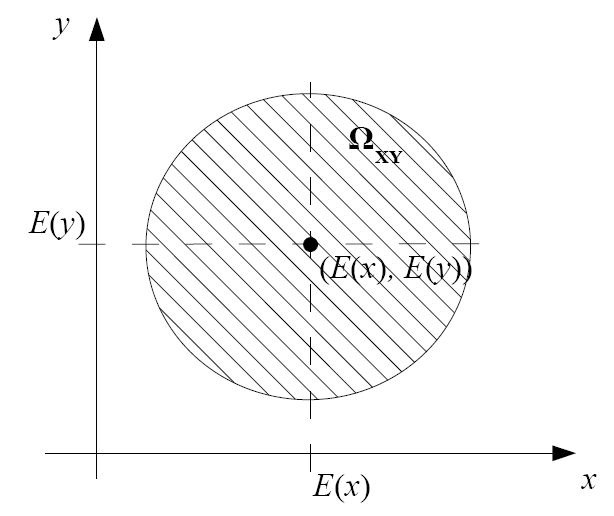
\includegraphics[width=5cm]{cov0.png} & 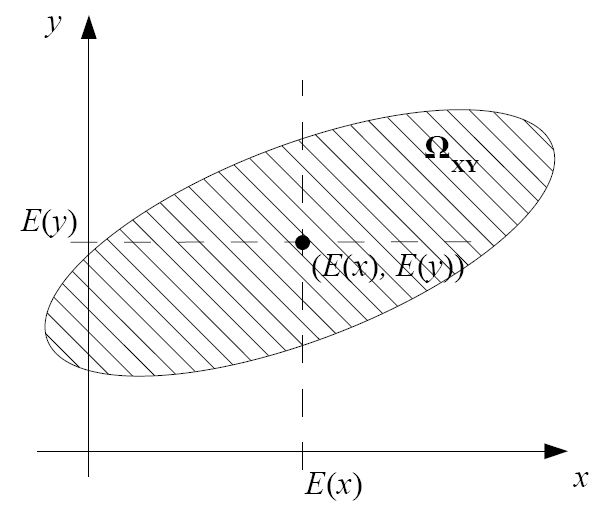
\includegraphics[width=5cm]{covpos.png} &
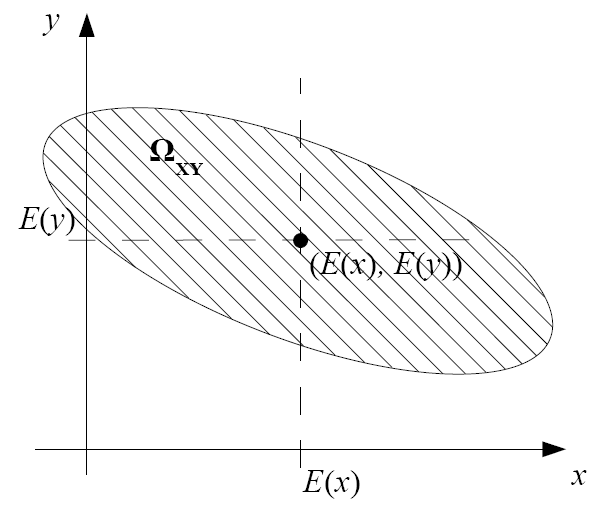
\includegraphics[width=5cm]{covneg.png} \\
$\mathrm{Cov}(X, Y)=0$ & $\mathrm{Cov}(X, Y) > 0$ & $\mathrm{Cov}(X, Y) < 0$ \\
$\rho_{XY}=0$ & $\rho_{XY}> 0$ & $\rho_{XY}< 0$
\end{tabular}
\end{center}
\end{figure}

\newpage
\begin{exemple}
(Exercici 10). La funci\'o de probabilitat conjunta de dues v.a. $X$ i $Y$ \'es
\[
\begin{array}{c|c|c|c|c|c|c}
X \backslash Y & 1 & 2 & 3 & 4 & 5 & 6\\ \hline
1 & 1/36 & 1/36 & 1/36 & 1/36 & 1/36 & 1/36 \\ \hline
2 & 0 & 2/36 & 1/36 & 1/36 & 1/36 & 1/36 \\ \hline
3 & 0 & 0 & 3/36 & 1/36 & 1/36 & 1/36 \\ \hline
4 & 0 & 0 & 0 & 4/36 & 1/36 & 1/36 \\ \hline
5 & 0 & 0 & 0 & 0 & 5/36 & 1/36 \\ \hline
6 & 0 & 0 & 0 & 0 & 0 & 6/36 \\ \hline
\end{array}
\]
\begin{enumerate}[a)]
\item Obteniu la funci\'o de probabilitat de $X$ condicionada a $Y=4$.
\item Quina \'es l'esperan\c{c}a de $X$ condicionada a $Y=4$?
\item I la vari\`ancia de $X$ condicionada a $Y=4$?
\end{enumerate}
\end{exemple}

\vskip 0.2 cm
\begin{exemple}
(Exercici 16cde).
Siguin $X$ i $Y$ dues variables aleat\`ories amb densitat
conjunta 
\[
f_{XY}(x,y) = \left\{\begin{array}{ll}\frac{1}{x} &
\mbox{si } 0 \leq y \leq x \leq 1\\ 0 & \mbox{en cas
contrari}\end{array}\right.
\]
\begin{enumerate}[a)]
\item Calculau $E(Y)$ 
\item Calculau $E(Y|X)$
\item Calculau $E(E(Y | X))$ i comprovau que coincideix amb $E(Y)$.
\end{enumerate}
\end{exemple}

\vskip 0.2 cm
\begin{exemple}
(Exercici 17bd)
Considerem un experiment amb tres possibles resultats $E_1,
E_2 \mbox{ i } E_3$ amb probabilitats respectives $p,q$ i $r$ tals
que $p+q+r = 1.$ En una seq\"{u}\`encia de $n$ proves independents de
l'experiment, denotem per $X$ el nombre de vegades que ocorr
$E_1$, i per $Y$ el nombre de vegades que ocorr $E_2$. Es sap que
el vector $(X,Y)$ t\'e una distribuci\'o anomenada \textbf{trinomial}
que ve donada per: $$P(X=i,Y=j) = {n! \over i! \> j! \> k!} \>
p^i \> q^j \> r^k \> , \ \ \ k = n-i-j$$
\begin{enumerate}[a)]
\item Determinau el vector mitjana i la matriu de covari\`ancies de
$(X,Y)$.
\item Obteniu l'expressi\'o de $E(Y | X = i) \ \ \forall i = 0,
 \ldots , n$.
\end{enumerate}

\end{exemple}

\vskip 0.2 cm
\begin{exemple}
(Exercici 20).
Es llan\c{c}a un dau sense biaix. Sigui $X$ la variable
aleat\`oria ``nombre de punts obtinguts", i $Y$ la variable aleat\`oria
que val 0 si s'obt\'e un 1, un 2 o un 3, i val 1 si s'obt\'e 4, 5 o 6.
Calculau la covari\`ancia  i el coeficient de
correlaci\'o  entre $X$ i $Y$.
\end{exemple}

\vskip 0.2 cm
\begin{exemple}
(Exercici 21)
La funci\'o de densitat conjunta de dues variables aleat\`ories
cont\'{\i}nues $X$ i $Y$ \'es: 
\[
f(x,y) = \begin{cases}
{3 \over 2}(x^2+y^2) & \text{si }  x,y \in (0,1)\\
0 & \text{en tot altre cas} \end{cases}
\]
Calculau les mitjanes, les vari\`ancies
, la covari\`ancia  i
el coeficient de correlaci\'o.
\end{exemple}


\vskip 1.5 cm
\noindent
Exercicis proposats: 18, 28, 22, 26

\end{document}